\documentclass{standalone}
\usepackage{tikz}
\usepackage{xcolor}
\usepackage{ifthen}
\usepackage{amsmath, amssymb}

\begin{document}

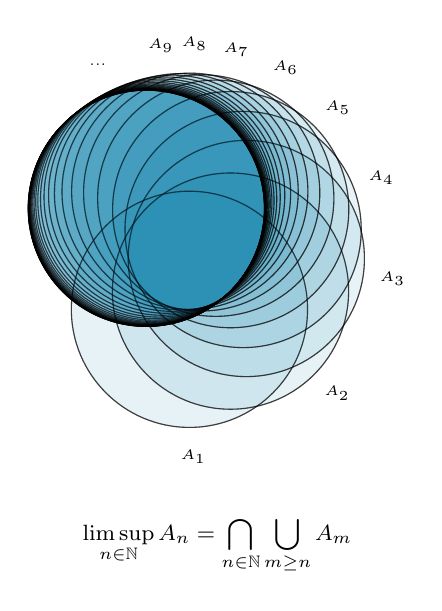
\begin{tikzpicture}[scale=1.5,]


    % Define colors
    \definecolor{lightgreen}{RGB}{34, 139, 34}
    \definecolor{bleudefrance}{rgb}{0.19, 0.55, 0.91}
    \definecolor{cerulean}{rgb}{0.0, 0.48, 0.65}

    % Set the distance of the circle centers from the origin
    \def\distance{0.5}

    % Set the radius of the circles
    \def\radius{1}

    % Define the angle range
    \def\startAngle{135}
    \def\endAngle{-135}
    \def\n{30} % Number of circles
    
    % Compute the angular step between circles
    \pgfmathsetmacro{\angleStep}{(\startAngle - \endAngle)/(\n-1)}

    % Draw the n circles from 135º to -135º
    \foreach \i in {1,...,\n} {
        \pgfmathsetmacro{\currentAngle}{\startAngle - (4/5)^\i*\n * \angleStep}
        \pgfmathsetmacro{\xCenter}{\distance * cos(\currentAngle)}
        \pgfmathsetmacro{\yCenter}{\distance * sin(\currentAngle)}
        
        % Draw each circle with the given radius
        \draw [draw opacity=0.5, fill opacity = 0.1 * (\n-\i+5)/(\n+5), fill = cerulean] (\xCenter, \yCenter) circle (\radius);
        \ifthenelse{\i<10}{
        \pgfmathsetmacro{\xLabel}{1.75 * cos(\currentAngle)};
        \pgfmathsetmacro{\yLabel}{1.75 * sin(\currentAngle)};
        \node at (\xLabel, \yLabel) {\tiny$A_{\i}$};
        }{
            \ifthenelse{\i=12}{
            \pgfmathsetmacro{\xLabel}{1.75 * cos(\currentAngle)};
            \pgfmathsetmacro{\yLabel}{1.75 * sin(\currentAngle)};
            \node at (\xLabel, \yLabel) {\tiny ...};
            }{}
        }
    }

        % Draw the n circles from 135º to -135º
        \foreach \i in {1,...,\n} {
            \pgfmathsetmacro{\currentAngle}{\startAngle - (4/5)^\i*\n * \angleStep}
            \pgfmathsetmacro{\xCenter}{\distance * cos(\currentAngle)}
            \pgfmathsetmacro{\yCenter}{\distance * sin(\currentAngle)}
            % Draw each circle with the given radius
            \draw [draw opacity=0.5] (\xCenter, \yCenter) circle (\radius);
        }
    
    \node at (0.25,-2.5) {\footnotesize $\displaystyle\limsup_{n \in \mathbb N} A_n = \bigcap_{n \in \mathbb N} \bigcup_{m \geq n} A_m $};

\end{tikzpicture}

\end{document}
